\documentclass[a4paper,12pt]{article}
\usepackage{cmap}
\usepackage[T2A]{fontenc}
\usepackage[utf8]{inputenc}
\usepackage[english,russian]{babel}
\usepackage{listings}
\usepackage{amsmath}
\usepackage{float}
\usepackage{csquotes}
\usepackage{graphicx}
\usepackage{xcolor}
\usepackage{hyperref}
\usepackage{mathtools}

\renewcommand{\theequation}{\thesection.\arabic{equation}}


\author{Шерепа Никита}
\title{ThinkDSP. Лабораторная 5. Автокорреляция.}
\date{\today}

\graphicspath{{res/screenshots}}

\begin{document}%
	
	\maketitle
	
	\newpage \tableofcontents
	\newpage \listoffigures
	\newpage \lstlistoflistings
	
	\newpage
	
	\definecolor{dkgreen}{rgb}{0,0.6,0}
	\definecolor{gray}{rgb}{0.5,0.5,0.5}
	\definecolor{mauve}{rgb}{0.58,0,0.82}
	
	\lstset{
		language=Python,                 % выбор ЯП для подсветки 
		basicstyle=\small\sffamily, % размер и начертание шрифта для подсветки кода
		numbers=left,               % где поставить нумерацию строк (слева\справа)
		numberstyle=\tiny,           % размер шрифта для номеров строк
		stepnumber=1,                   % размер шага между двумя номерами строк
		numbersep=5pt,                % как далеко отстоят номера строк от подсвечиваемого кода
		aboveskip=3mm,
		belowskip=3mm,
		showstringspaces=false,
		columns=flexible,
		captionpos=b, 
		basicstyle={\small\ttfamily},
		numbers=left,
		numberstyle=\tiny\color{gray},
		keywordstyle=\color{blue},
		commentstyle=\color{mauve},
		stringstyle=\color{dkgreen},
		breaklines=true,
		breakatwhitespace=true,
		tabsize=3
	}


	\section{Упражнение 5.1}
	
	\begin{enumerate}
		
		
		\item \textbf{Задание}
		
		Вычислите автокорреляцию для различных \textit{lag}, воспользовавшись материалами из \textit{chap05.ipynb}. Оцените высоты тона вокального чирпа для нескольких времен начала сегмента. 
		
		\item \textbf{Ход работы}
		
		Воспользуемся некоторыми методами из \textit{chap05.ipynb}
		
		
		\textit{serial\_corr} - вычисляет корреляцию для разных типов шума 
		\begin{lstlisting}[caption=Метод serial\_corr]
			def serial_corr(wave, lag=1):
			N = len(wave)
			y1 = wave.ys[lag:]
			y2 = wave.ys[:N-lag]
			corr = np.corrcoef(y1, y2)[0, 1]
			return corr
		\end{lstlisting}
		
		\textit{autocorr} - вызывает \textit{serial\_corr} с различными значениями \textit{lag} 
		\begin{lstlisting}[caption=Метод autocorr]
			def autocorr(wave):
			lags = np.arange(len(wave.ys)//2)
			corrs = [serial_corr(wave, lag) for lag in lags]
			return lags, corrs
		\end{lstlisting}
		
		Теперь возьмем звук, выберем из него фрагмент и найдем высоту его тона.
		\begin{lstlisting}[caption=Фрагмент 1 и высота его тона]
			wave = read_wave('res/28042__bcjordan__voicedownbew.wav')
			wave.normalize()
			segment = wave.segment(start=0.3, duration=0.01)
			
			lags, corrs = autocorr(segment)
			plt.plot(lags, corrs)
			decorate(xlabel='Lag (index)', ylabel='Correlation')
		\end{lstlisting}
		\begin{figure}[H]
			\centering
			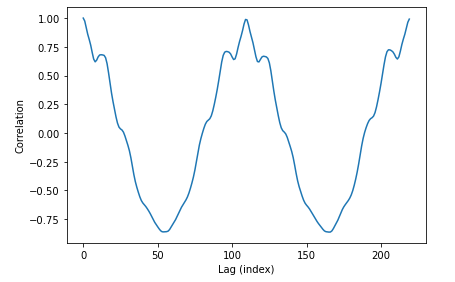
\includegraphics[width=0.75\textwidth]{1_1.png}
			\caption{Высота тона звука}
			\label{fig:1.1}
		\end{figure}
		
		Видим, что пик лежит между 100 и 120.
		Для уточнения \textit{lag} воспользуемся методом \textit{argmax}
		\begin{lstlisting}[caption=Уточнение частоты]
			low, high = 100, 120
			lag = np.array(corrs[low:high]).argmax() + low
			
			period = lag / segment.framerate
			frequency = 1 / period
			frequency
			
			Output
			404.5871559633028
		\end{lstlisting}
		Частота = 404.5871559633028
			
		Теперь возьмем другой фрагмент и вычислим частоту для него
		\begin{lstlisting}[caption=Фрагмент 2 и высота его тона]
			wave = read_wave('res/28042__bcjordan__voicedownbew.wav')
			wave.normalize()
			segment = wave.segment(start=0.6, duration=0.01)
			
			lags, corrs = autocorr(segment)
			plt.plot(lags, corrs)
			decorate(xlabel='Lag (index)', ylabel='Correlation')
		\end{lstlisting}
		\begin{figure}[H]
			\centering
			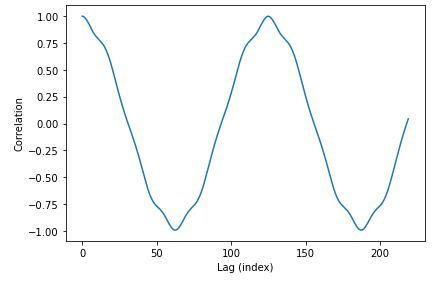
\includegraphics[width=0.75\textwidth]{1_2.png}
			\caption{Высота тона звука}
			\label{fig:1.2}
		\end{figure}
		
		Видим, что пик лежит между 100 и 150.
		Для уточнения \textit{lag} воспользуемся методом \textit{argmax}
		\begin{lstlisting}[caption=Уточнение частоты]
			low, high = 90, 110
			lag = np.array(corrs[low:high]).argmax() + low
			
			period = lag / segment.framerate
			frequency = 1 / period
			frequency
			
			
			Output
			352.8
		\end{lstlisting}
		Частота = 352.8
		
		Частота уменьшается с увеличением времени начала сегмента.
		
	\end{enumerate}
	\newpage


	\section{Упражнение 5.2}
	
	\begin{enumerate}
		
		
		\item \textbf{Задание}
		
		Инкапсулируйте код, выполняющий автокорееляцию в функцию, названную \textit{estimate\_fundamental}, и используйте её для отслеживания высоты тона записанного звука.
		
		Проверьте, насколько хороша она работает, накладывая оценки высоты тона на спектрограмму записи.
		
		\item \textbf{Ход работы}
		
		Возьмём звук из прошлого пункта и построим его спектрограмму
		\begin{lstlisting}[caption=Спектрограмма звука]
			from thinkdsp import read_wave
			
			wave = read_wave('res/28042__bcjordan__voicedownbew.wav')
			wave.normalize()
			
			wave.make_spectrogram(2048).plot(high=4200)
			decorate(xlabel='Time (s)', 
			ylabel='Frequency (Hz)')
		\end{lstlisting}
		\begin{figure}[H]
			\centering
			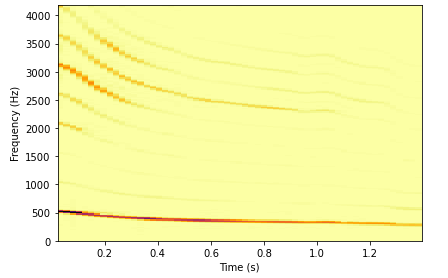
\includegraphics[width=0.75\textwidth]{2_1.png}
			\caption{Спектрограмма звука}
			\label{fig:2.1}
		\end{figure}
	
	
		Теперь инкапсулируем код в функцию \textit{estimate\_fundamental}
		\begin{lstlisting}[caption=Метод \textit{estimate\_fundamental}]
			def estimate_fundamental(segment, low = 70, high = 150):
			lags, corrs = autocorr(segment)
			lags = np.array(corrs[low:high]).argmax() + low
			period = lag / segment.framerate
			frequency = 1 / period
			return frequency
		\end{lstlisting}
		
		Проверим его работоспособность
		\begin{lstlisting}[caption=Вычисление частоты с помощью метода \textit{estimate\_fundamental}]
			segment = wave.segment(start = 0.2, duration = 0.01)
			frequency = estimate_fundamental(segment)
			frequency
			
			Output
			436.63366336633663
		\end{lstlisting}
	
		Частота = 436.63366336633663
		
		Теперь вычислим высоту тона записанного звука и построим кривую отслеживания тона, наложенную на спектрограмму
		\begin{lstlisting}[caption=Вычисление кривой отслеживания тона]
			step = 0.05
			starts = np.arange(0.0, 1.4, step)
			duration = 0.01
			
			ts = []
			freqs = []
			
			for start in starts:
			ts.append(start + step/2)
			segment = wave.segment(start, duration)
			freq = estimate_fundamental(segment)
			freqs.append(freq)
			
			wave.make_spectrogram(2048).plot(high=900)    
			plt.plot(ts, freqs, color='green')
			decorate(xlabel='Time (s)', 
			ylabel='Frequency (Hz)',
			xlim=[0, 1.4],
			ylim=[0, 900])
		\end{lstlisting}
		\begin{figure}[H]
			\centering
			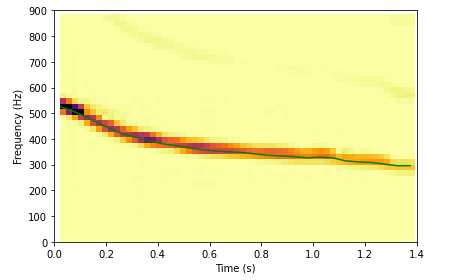
\includegraphics[width=0.75\textwidth]{2_2.png}
			\caption{Кривая и спектрограмма}
			\label{fig:2.2}
		\end{figure}
		Видим, что зеленая кривая правильно наложилась на спектрограмму, значит все вычисления верны.
		
	\end{enumerate}
	\newpage
	
	
	\section{Упражнение 5.3}
	
	\begin{enumerate}
		
		
		\item \textbf{Задание}
		
		Используя данные про \textit{BitCoin} из прошлой лабораторной работы, вычислите автокорреляции цен в платежной системе \textit{BitCoin}. Быстро ли спадает автокорреляционная функция? Есть ли признаки периодичности процесса?
		
		\item \textbf{Ход работы}
		
		Вспомним данные про \textit{BitCoin} из прошлой лабораторной работы
		\begin{lstlisting}[caption=Таблица цен \textit{BitCoin}]
			import pandas as pd
			
			df = pd.read_csv('res/BTC_USD_2013-10-01_2021-05-05-CoinDesk.csv', 
			parse_dates=[0])
			df
		\end{lstlisting}
		\begin{figure}[H]
			\centering
			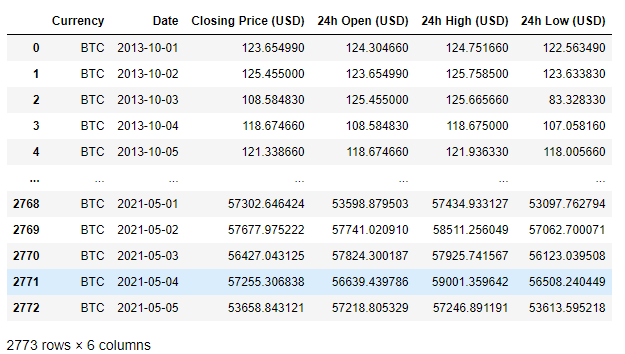
\includegraphics[width=0.75\textwidth]{3_1.png}
			\caption{Таблица цен \textit{BitCoin}}
			\label{fig:3.1}
		\end{figure}
		
		\begin{lstlisting}[caption=График цен \textit{BitCoin}]
			ys = df['Closing Price (USD)']
			ts = df.index
			
			from thinkdsp import Wave
			
			wave = Wave(ys, ts, framerate=1)
			wave.plot()
			decorate(xlabel='Time (days)')
		\end{lstlisting}
		\begin{figure}[H]
			\centering
			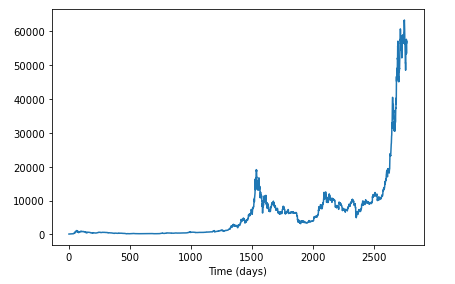
\includegraphics[width=0.75\textwidth]{3_2.png}
			\caption{График цен \textit{BitCoin} за 7 лет}
			\label{fig:3.2}
		\end{figure}
	
	
		Теперь воспользуемся функцией автокорреляции
		\begin{lstlisting}[caption=Автокоррелируем]
			lags, corrs = autocorr(wave)
			plt.plot(lags, corrs)
			decorate(xlabel='Lag',
			ylabel='Correlation')
		\end{lstlisting}
		\begin{figure}[H]
			\centering
			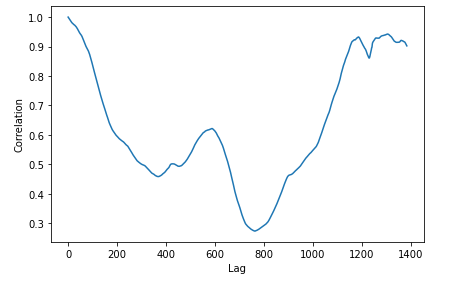
\includegraphics[width=0.75\textwidth]{3_3.png}
			\caption{Результат автокорреляции}
			\label{fig:3.3}
		\end{figure}
		
		Как видим, идет плавное уменьшение значения, как у розового шума. Результат совпадает с результатом прошлом лабораторной.
		
		Увеличение значения происходит из-за того, что на самом графике курс цен сначала увеличился, а затем уменьшился, а затем опять резко увеличился.
		
		
	\end{enumerate}
	\newpage
	
	
	\section{Упражнение 5.4}
	
	\begin{enumerate}
		
		
		\item \textbf{Задание}
		
		Поэкспериментируйте с исследованием автокорреляции, используя материалы файла \textit{saxophone.ipynb}
		
		\item \textbf{Ход работы}
		
		Вопроизведем звук саксофона и посмотрим на спектр сигнала вблизи
		\begin{lstlisting}[caption=Работа со звуком]
			from thinkdsp import read_wave
			
			wave = read_wave('res/100475__iluppai__saxophone-weep.wav')
			wave.normalize()
			wave.make_audio()
			
			start = 2.0
			duration = 0.5
			segment = wave.segment(start=start, duration=duration)
			segment.make_audio()
			
			spectrum = segment.make_spectrum()
			spectrum.plot(high=3000)
			decorate(xlabel='Frequency (Hz)', ylabel='Amplitude')
		\end{lstlisting}
		\begin{figure}[H]
			\centering
			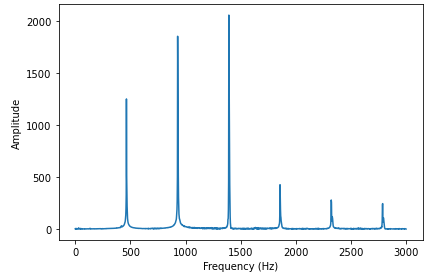
\includegraphics[width=0.75\textwidth]{4_1.png}
			\caption{Спектр сигнала с 2 по 2.5 секунду}
			\label{fig:4.1}
		\end{figure}
	
		Воспринимаем мы основную частоту, равную 464 Гц. Но она не доминирующая. Доминирующая = 1392 Гц.
		
		Воспользуемся автокорреляцией, чтобы понять, почему мы воспринимаем не доминирующую частоту.
		
		\begin{lstlisting}[caption=Автокоррелируем]
			def autocorr(segment):
				corrs = np.correlate(segment.ys, segment.ys, mode='same')
				N = len(corrs)
				lengths = range(N, N//2, -1)
				
				half = corrs[N//2:].copy()
				half /= lengths
				half /= half[0]
				return half
				
			corrs = autocorr(segment)
			plt.plot(corrs[:200])
			decorate(xlabel='Lag', ylabel='Correlation', ylim=[-1.05, 1.05])
		\end{lstlisting}
		\begin{figure}[H]
			\centering
			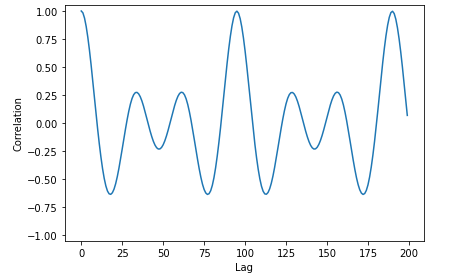
\includegraphics[width=0.75\textwidth]{4_2.png}
			\caption{Результат автокорреляции}
			\label{fig:4.2}
		\end{figure}
		
		Как видим, первый крупный пик находится в районе lag = 100
		
		Воспользуемся фнукцией, которая находит самую высокую корреляцию в заданном диапазоне задержек и возвращает соответствующую частоту - \textit{find\_frequency}
		
		\begin{lstlisting}[caption=Функция \textit{find\_frequency}]
			def find_frequency(corrs, low, high):
			lag = np.array(corrs[low:high]).argmax() + low
			print(lag)
			period = lag / segment.framerate
			frequency = 1 / period
			return frequency
		\end{lstlisting}
		
		Вычислим частоту 1ого пика
		\begin{lstlisting}[caption=Частота первого пика]
			find_frequency(corrs, 80, 100)
			
			Output
			464.2105263157895
		\end{lstlisting}
		Частота = 464.2105263157895
		
		Если попробовать удалить частоту 464 Гц из спектра то восприятие не изменится
		\begin{lstlisting}[caption=Удалим частоту 464 Гц]
			spectrum2 = segment.make_spectrum()
			spectrum2.high_pass(600)
			spectrum2.plot(high=3000)
			decorate(xlabel='Frequency (Hz)', ylabel='Amplitude')
		\end{lstlisting}
		\begin{figure}[H]
			\centering
			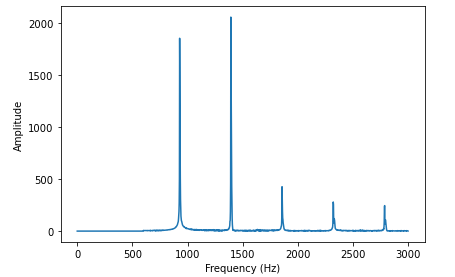
\includegraphics[width=0.75\textwidth]{4_3.png}
			\caption{Удалили частоту 464 Гц}
			\label{fig:4.3}
		\end{figure}
		
		Всопринимается всё еще частота = 464 Гц. Это явление называется \textit{"подавленная" основная частота}.
		
		Мы всё еще восприминаем частоту = 464 Гц, потому что оставшиеся пики, которые присутствуют в сигнале, представляют собой гармоники 464 Гц.
		
		Наше ухо интерпретирует высокие гармоники как свидетельство того, что «правильная» основная частота = 464 Гц.
		
		Если избавиться от остальных пиков, то весь эффект пропадет и мы будем слышать не саксофон, а звук, похожий на сигнал перед записью сообщения на автоответчик.
		
		\begin{lstlisting}[caption=Убираем пики]
			spectrum4 = segment.make_spectrum()
			spectrum4.high_pass(600)
			spectrum4.low_pass(1200)
			spectrum4.plot(high=3000)
			decorate(xlabel='Frequency (Hz)', ylabel='Amplitude')
		\end{lstlisting}
		\begin{figure}[H]
			\centering
			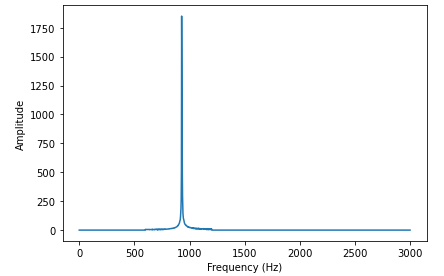
\includegraphics[width=0.75\textwidth]{4_4.png}
			\caption{Убрали пики}
			\label{fig:4.3}
		\end{figure}
		
		
		
	\end{enumerate}
	\newpage
	
	
	\section{Вывод}
		
	В результате выполнения лабораторной работы получены навыки работы с корреляцией, автокорреляцией. Мы ознакомились с явлением "подавленных" основных частот и функцией автокорреляции.
		
	\newpage
	
\end{document}